\markboth{CAPITOLO 6. ESERCIZI A.A. 2017-18}{CAPITOLO 6. ESERCIZI A.A. 2017-18}
\begin{flushleft}

\bigskip
\textbf{Esercizio 6.1} \textit{Scrivere una function Matlab che generi la matrice \textit{sparsa} $n \times n$, con $n > 10$\\
$$
A_n = \begin{pmatrix} a_{11} & \ldots & a_{1n} \\ \vdots & & \vdots \\ a_{n1} & \ldots & a_{nn}\end{pmatrix}, \qquad \text {con } \qquad a_{ij} \begin{cases} 4 \text{ se } i = j \\ -1 \text{ se } i = j \pm 1 \\ -1 \text{ se } i = j \pm 10\end{cases}
$$
Utilizzare a questo fine la function Matlab \lstinline{spdiags}.}\\
\textbf{Soluzione: }
\lstinputlisting[language=Matlab]{Capitolo6/es6_1.m}
\bigskip
\textbf{Esercizio 6.2} \textit{	Utilizzare il metodo delle potenze per calcolare l'autovalore dominante della matrice $A_n$ del precedente esercizio, con una approssimazione $tol=10^{-5}$, partendo da un vettore con elementi costanti. Riempire, quindi, la seguente tabella: \\ \begin{center}
\begin{tabular}{ | l | c | r |}
	\hline
	$n$ & \textit{numero iterazioni effettuate} & \textit{stima autovalore} \\ \hline
	100 &  &  \\ \hline
	\vdots &  &  \\  \hline
1000 &  &  \\
	\hline
\end{tabular}
\end{center}}
\textbf{Soluzione: }La tabella richiesta � la seguente:\\
\[
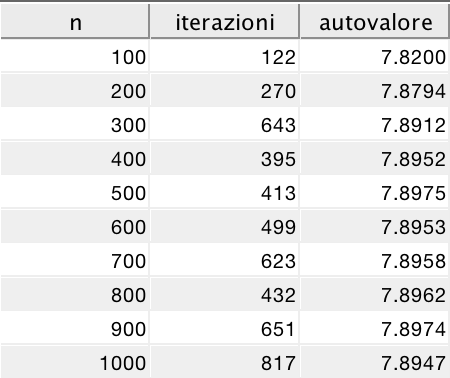
\includegraphics[scale=0.4]{Capitolo6/es6_2.png}
\]
Generata grazie al seguente codice matlab:
\lstinputlisting[language=Matlab]{Capitolo6/es6_2.m}
\newpage
\textbf{Esercizio 6.3} \textit{	Utilizzare il metodo di Jacobi per risolvere il sistema lineare\\
	\[
	A_n \textbf{x} = \begin{pmatrix} 1 \\ \vdots \\ 1 \end{pmatrix},
	\]
	dove $A_n$ � la matrice definita in (1), con tolleranza $tol=10^{-5}$, e partendo dal vettore nullo. Graficare il numero di iterazioni necessarie, rispetto alla dimensione $n$ del problema, con $n$ che varia da 100 a 1000 (con passo 20).}\\
\textbf{Soluzione: }
\[
	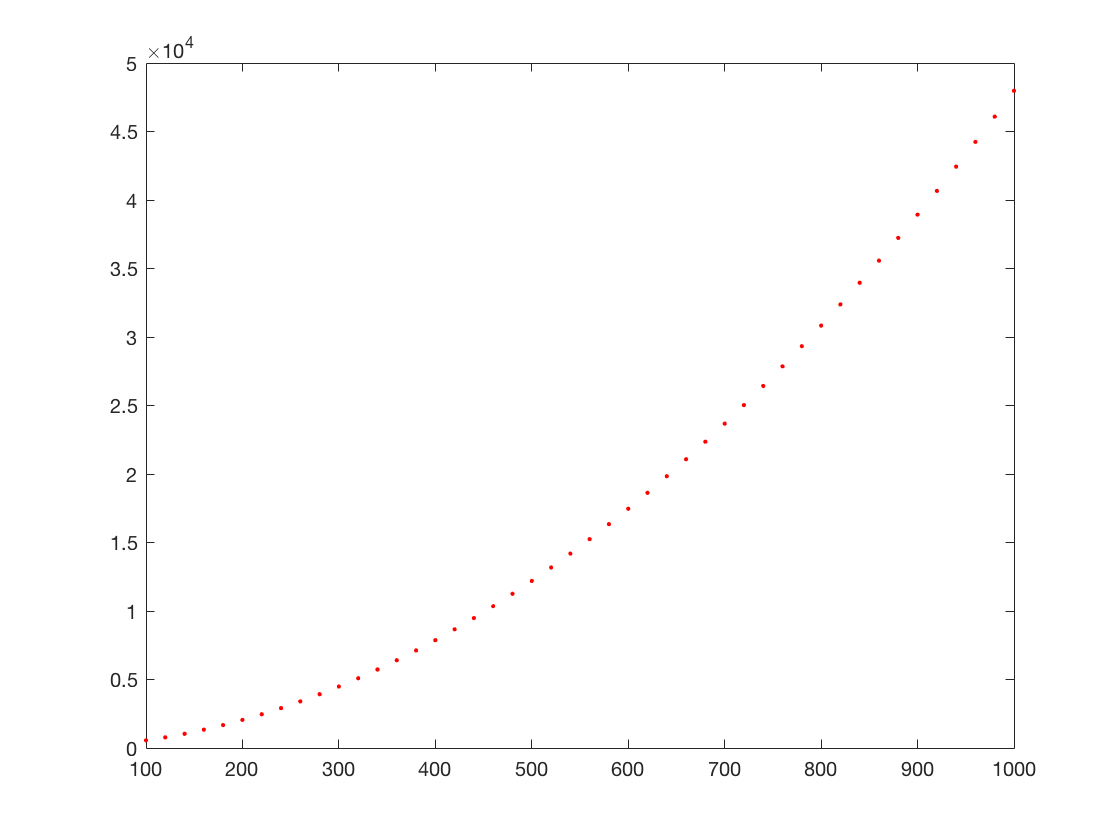
\includegraphics[scale=0.35]{Capitolo6/es6_3.png}
\]
Il codice matlab che ha generato il grafico:
\lstinputlisting[language=Matlab]{Capitolo6/es6_3.m}

\bigskip
\textbf{Esercizio 6.4} \textit{ Ripetere una procedura analoiga a quella del precedente esercizio utilizzando il metodo di Gauss-Seidel.}\\
\textbf{Soluzione: }
\[
	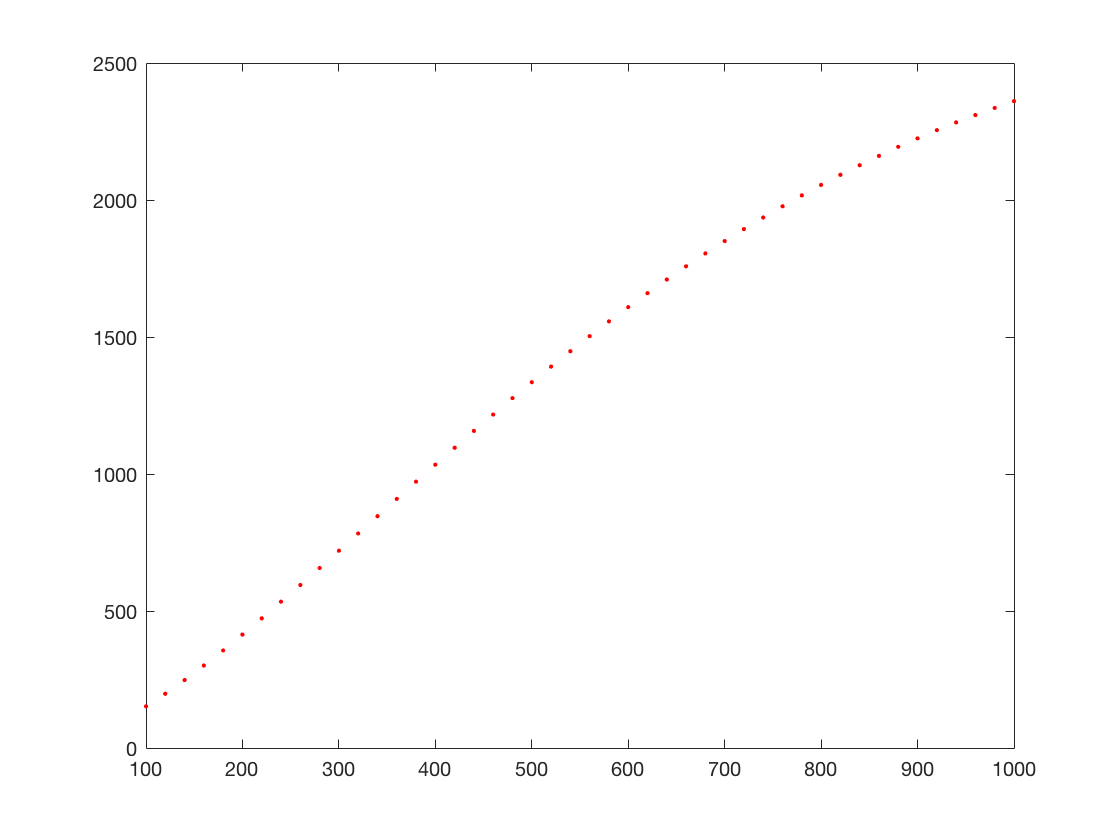
\includegraphics[scale=0.35]{Capitolo6/es6_4.png}
\]
Il codice matlab che ha generato il grafico:
\lstinputlisting[language=Matlab]{Capitolo6/es6_4.m}
\newpage
\textbf{Esercizio 6.5} \textit{
Con riferimento al sistema lineare (2), con $n=1000$, graficare la norma dei residui rispetto all'indice di iterazione, generati dai metodi di Jacobi e Gauss-Seidel. Utilizzare il formato \lstinline{semilogy} per realizzare il grafico, corredandolo di opportune $label$.}
\textbf{Soluzione: }
Il seguente grafico � realizzato con le ascisse in scala logaritmica tramite il formato semilogaritmico semilogy di Matlab:
\[
	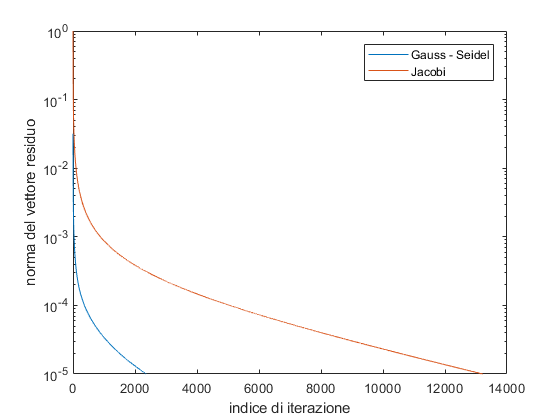
\includegraphics[scale=0.85]{Capitolo6/es6_5.png}
\]
Il codice matlab che ha generato il grafico:
\lstinputlisting[language=Matlab]{Capitolo6/es6_5.m}

\end{flushleft}
